\vspace{-5pt}
\section{Monster Munch Pilot Study}
Because the Data Collection Phase was used to populate data in the community board, and therefore the creation of the app, the report of the users from the collection phase will not be mentioned moving forward. See Figure~\ref{fig:phasechart} for details.

%The pilot with Monster Munch was conducted with participants recruited via both Amazon Mechanical Turk (AMT) and social media sites. 
The goals of the pilot study were to (1) to assess users general perceptions using a lightweight app for engaging with nutrition and (2) understand how the different gamification and social mechanisms built into the app (avatars and crowdsourced community board) shape users preferences and experience with the app. The pilot study followed the procedure outlined below and summarized in Figure~\ref{fig:studyflow}. 


\begin{figure}[ht]
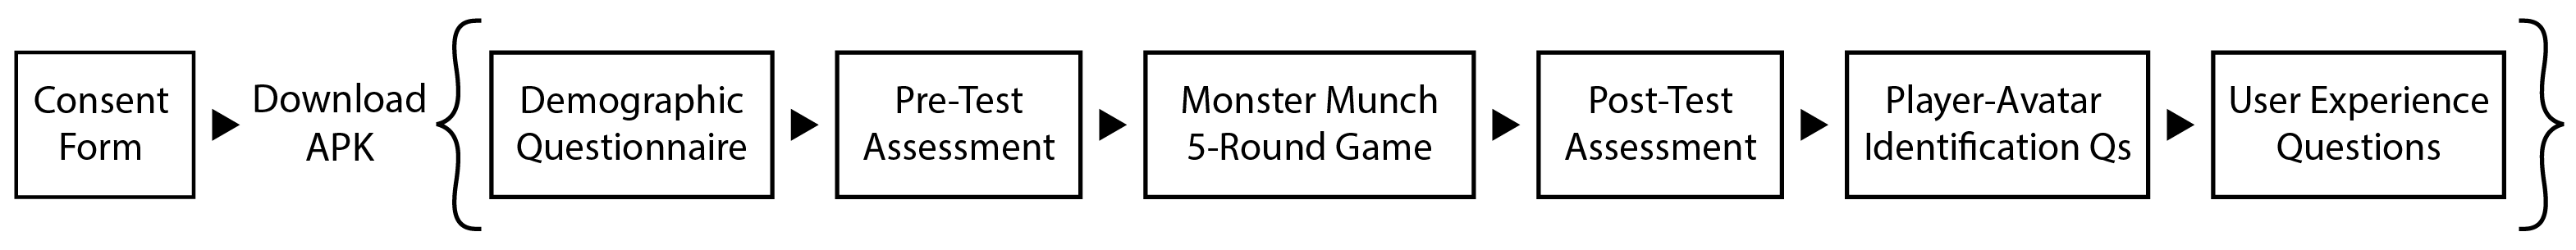
\includegraphics[width=\textwidth]{samples/images/figure-1.png}
\caption{Study flow for participants in the Monster Munch pilot study. Study sections indicated inside the curly braces were completed within the mobile app. }
\label{fig:studyflow}
\end{figure}

\vspace{-5pt}
\subsection{Participant Recruitment}
Participants were recruited from Amazon Mechanical Turk and social media sites (Facebook and Instagram). Users were screened with the following inclusion criteria: 1) own an Android mobile device, 2) above 18 years of age. After accepting the terms of the study found in the consent form, participants  downloaded an APK file and installed the Monster Munch app. Within the app they completed (1) a pre-test evaluation, (2) Monster Munch nutrition activities, and (3) post-test evaluation. Only participants who completed all three tasks were considered in subsequent analyses. 


\vspace{-5pt}
\subsection{Monster Munch App Activities}

In the Monster Munch app, users could view each of the four pet monster avatars and their nutritional goals before selecting one to proceed with and ``help'' during the app. Users also had the opportunity to give their monster a custom name before completing the task and helping feed their monster.

In the core monster feeding task, users selected meals to feed their chosen monster for five rounds. Each round of meal selection consisted of five steps. 
First, the user was presented with  four options of ``in-the-wild'' meal photographs, accompanied with brief descriptions of the contents of each meal that they could review to decide what to feed their monster. Second, users were asked to select the meal that they believed best fit their monster’s nutritional goal and provide a short text-based description of why they selected that particular option. Third, users viewed the crowdsourced community board (CB) where they could consider which meal other members of the community chose to feed their monster. Users could view the percent of users that selected each meal and their reasoning for doing so (these percents and rationales were sourced from the data collection phase described above). Fourth, armed with this new information, users had the option to keep their original meal selection, or switch to another meal option. Again, users were asked to provide a short description to rationalize their final meal selection after viewing the input from the CB.
Finally, after they submitted their reasoning, the app told the user whether the meal option they selected was (in)correct, and which meal option was the best choice. The appearance of the monster avatar also changed in response to the user's performance, becoming ``healthier'' if the user selected the correct meal, and ``less healthy'' if the user selected the incorrect meal. 
Users repeated these steps for five meal selection rounds with the same  monster avatar, helping them work towards their monster's nutritional goal.
\vspace{-5pt}
\subsection{Data Analysis and Measures of Interest}
Participants' survey responses were collected via Qualtrics and their engagement with the app  collected via the Google Cloud computing platform Firebase and extracted with Python 2.7. Users' data from Qualtrics and Firebase were merged together for processing, and 
%\url{https://github.com/mlhwang/m4m}
Statistical Package for the Social Sciences (SPSS version 27) was used to analyze the data. For all analysis the alpha significance threshold was set at 0.05.  

\subsubsection{Player Avatar Identification}
Users' engagement with the gamified avatar component of the task was assessed with four Player Avatar Identification (PAID) questions asked in the post-task survey (adapted from~\cite{li2013player}). Users indicated their agreement to the following four statements on a 7-point Likert scale (with the option to select ``Not Applicable''): 
\begin{enumerate}
    \item ``When my monster’s condition worsened, I felt angry/sad.''
    \item ``When my monster achieved their goals, I felt happy.''
    \item ``My monster reflects who I am.''
    \item ``My monster influences the way I feel about myself.'' 
\end{enumerate}
A ``PAID score'' was calculated for each user by summing their responses to each question. Higher PAID scores indexed stronger player-avatar identification.

\subsubsection{Community Board (CB) Agreement}

The CB was created through the Data Collection Phase. The two CB related questions during the post-app task included: 
\begin{enumerate}
    \item ``Did the community board influence your final meal choice?'' 
    \item ``How often did you agree with the rest of the community?'
\end{enumerate}

Users responded on a scale of `Always;' `More than half of the time;' `About half of the time;' `Less than half of the time;' `Never;' and `I did not look at the community board.' 

\subsubsection{Macronutrient Knowledge Assessment}
%the inclusion of a baseline and post-task nutritional assessment allowed us to investigate preliminary measurements to see if Monster Munch might relate to improved recollection of nutritional information and indicate that the app has the potential to become a future learning tool. 
In order to see if Monster Munch might relate to improved recollection of nutritional information, macronutrient knowledge was evaluated before and after the Monster Munch app activities. The percentage correct was calculated for the 12-question pre-test to establish a baseline for nutritional knowledge. After using the Monster Munch app, users completed an 18-question post-test, 12 repeated-questions and six new questions. Performance on the 12 repeated questions was used to assess recall of nutrition knowledge, and performance on the six new questions was used to assess transfer of nutrition knowledge in comparison to the baseline evaluation. 
\vspace{-5pt}
\subsection{Research Questions}
In the next section we discuss the results from this pilot study using Monster Munch. In particular this pilot evaluation was centered around understanding the following questions:
\begin{enumerate}
    \item Does playing Monster Munch influence users' confidence of their ability to estimate macronutrient content of ``in-the-wild'' meal photographs (a proxy for nutritional engagement)?
    \item Does the inclusion of gamification and social mechanisms (pet monster avatars and crowdsourced community board) influence enjoyment/engagement of the Monster Munch app?
    \item Do gamification and social mechanisms have an effect on nutritional learning?
\end{enumerate}

% The hypotheses are:
% \begin{itemize}
%     \item \textbf{H1}: User's will report higher enjoyment and show greater engagement with the Monster Munch app after the inclusion of Gamification Mechanisms. 
%     \item \textbf{H2}: Monster Munch (a mobile app for nutritional engagement) will help users become more confident in their ability to assess macronutrient content of ``in-the-wild'' meal photographs pre- to post-test.
%     \item \textbf{H3}: Users who chose pet avatars with a health goal that is personally meaningful in Monster Munch are more likely to perform better (i.e., identify the right meal photographs for a specific nutritional goal) pre- to post-test.

% \end{itemize}

 



